\section{Results}

\subsection{Phase 2D Interpretation Audit}

The Phase 2D audit supports a narrowed interpretation. P3 grouped sparse points fail against both random-coordinate and alternative-reference controls. P4 privileged union boxes remain positive, showing that the broad SAM backbone failure claim would be too strong. Table~\ref{tab:control_decomposition} decomposes the C1/C2 controls and relabels C2 as an alternative-reference control for scientific discussion, without modifying the original historical CSVs.

\begin{table*}[t]
\centering
\small
\caption{C1/C2 decomposition over all Phase 2D prompt families. C2 is retained historically but interpreted as an alternative-reference control.}
\label{tab:control_decomposition}
\begin{tabular}{llllll}
\hline
Segmenter & Prompt & P - C1 & P - C2 & C1 - C2 & C2 label \\
\hline
SAM-B & P1 & -0.043 & -0.096 & -0.053 & alternative\_reference\_control \\
SAM-B & P2 & -0.084 & -0.043 & 0.041 & alternative\_reference\_control \\
SAM-B & P3 & -0.160 & -0.156 & 0.003 & alternative\_reference\_control \\
SAM-B & P4 & 0.044 & 0.064 & 0.020 & alternative\_reference\_control \\
SAM-B & P5 & -0.201 & -0.099 & 0.102 & alternative\_reference\_control \\
SAM-L & P1 & 0.082 & -0.058 & -0.141 & alternative\_reference\_control \\
SAM-L & P2 & 0.001 & 0.012 & 0.011 & alternative\_reference\_control \\
SAM-L & P3 & -0.074 & -0.119 & -0.045 & alternative\_reference\_control \\
SAM-L & P4 & 0.039 & 0.095 & 0.056 & alternative\_reference\_control \\
SAM-L & P5 & 0.049 & -0.016 & -0.065 & alternative\_reference\_control \\
\hline
\end{tabular}
\end{table*}


\begin{figure}[t]
\centering
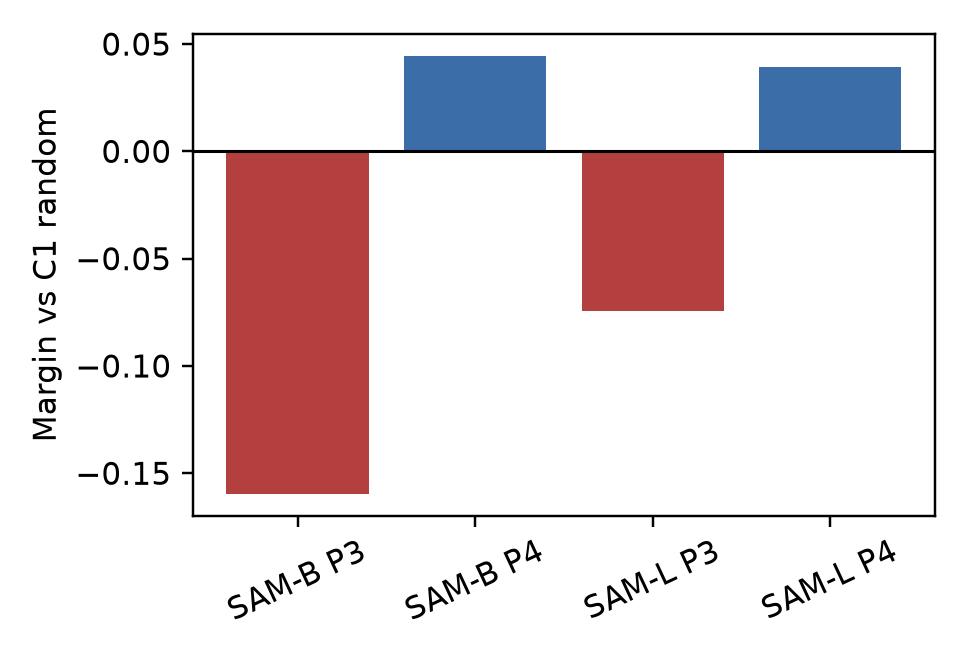
\includegraphics[width=\columnwidth]{figures/phase2d_point_vs_region_upper_bound.png}
\caption{P3 grouped points have negative margins, while privileged P4 region boxes are positive. This motivates a region-prompt pivot but does not establish an automatic method.}
\label{fig:p3_p4}
\end{figure}

\begin{figure}[t]
\centering
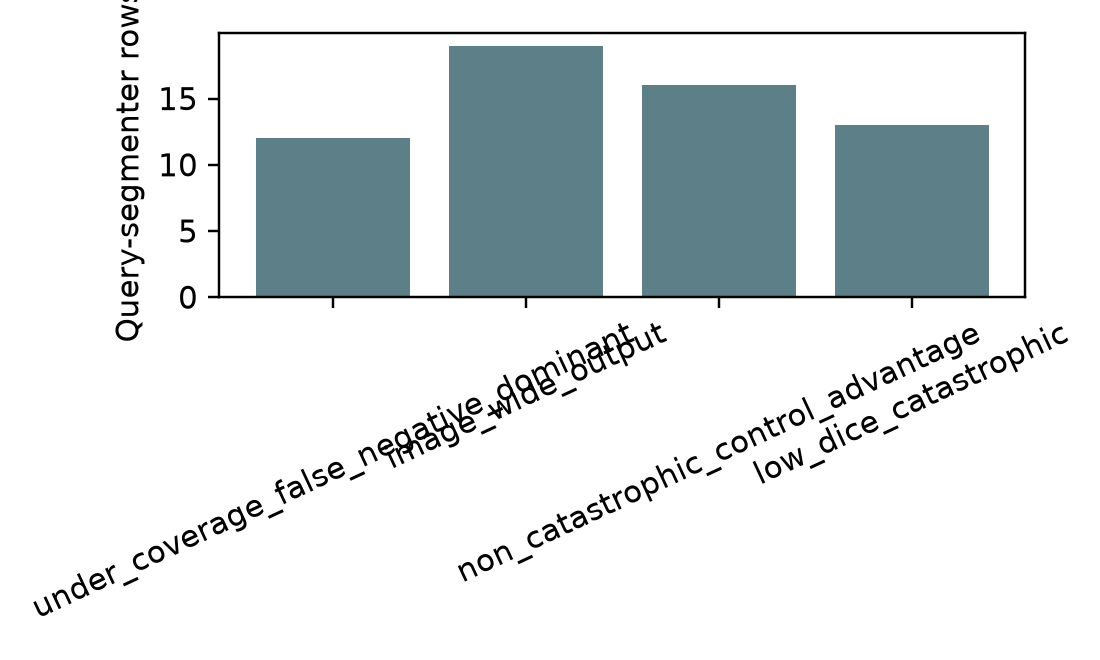
\includegraphics[width=\columnwidth]{figures/p3_failure_taxonomy.png}
\caption{P3 failure taxonomy from existing Phase 2D artifacts. Failure modes include under-coverage and image-wide outputs, consistent with a prompt-interface problem.}
\label{fig:p3_failure_taxonomy}
\end{figure}

\begin{figure*}[t]
\centering
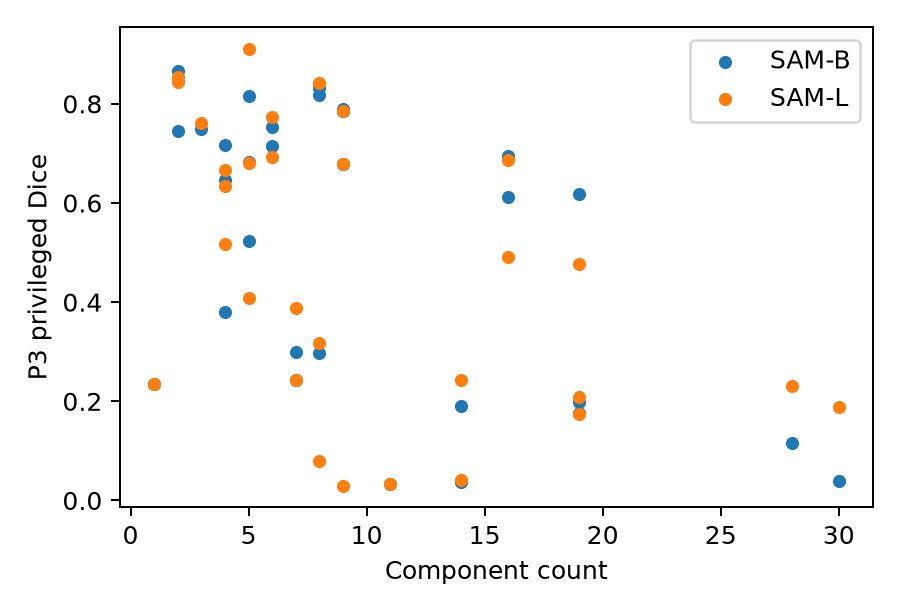
\includegraphics[width=.48\textwidth]{figures/phase2d_dice_vs_component_count.png}
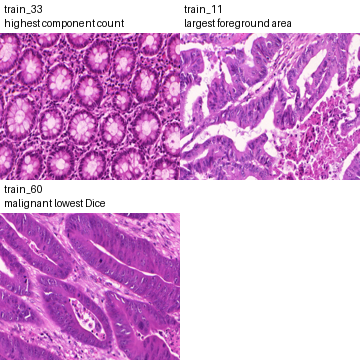
\includegraphics[width=.48\textwidth]{figures/phase2d_representative_failure_panels.png}
\caption{Existing Phase 2D failure diagnostics reused without new SAM inference. Left: grouped-point Dice varies with component structure. Right: representative failure panels selected by the Phase 2D audit rule, not by post-hoc favorable case selection.}
\label{fig:phase2d_failure_panels}
\end{figure*}

These visual diagnostics are included to prevent an overly broad backbone-failure interpretation. Some failures are under-coverage errors, where the grouped point interface captures only sparse parts of a whole-image gland mask. Other failures are image-wide outputs, where the prompt interface does not constrain SAM in a useful way. In both cases, the failure is compatible with a bad prompt representation even when the coordinate and cost audits pass.

\subsection{Gate R1 Proposal Quality}

Table~\ref{tab:r1_quality} reports the strict-validation Gate R1 results. No automatic family passes. R03 automatic union box is the strongest route by mean metric, but its improvement over size-matched random boxes is only 0.026 and its win rate is 0.200. R00 direct matching mask is precise but has low recall and low raw Dice. R04 and R05 are too small and under-cover glands.

\begin{table*}[t]
\centering
\small
\caption{Gate R1 proposal quality on 30 strict-validation queries. No automatic family passed the pre-registered thresholds.}
\label{tab:r1_quality}
\begin{tabular}{lllllllll}
\hline
Family & Route & Metric & Control & Improvement & Win & Recall & Empty & Status \\
\hline
R00 direct matching mask & mask & 0.179 & 0.595 & -0.416 & 0.067 & 0.100 & 0.000 & FAIL \\
R03 automatic union box & box & 0.745 & 0.719 & 0.026 & 0.200 & 0.791 & 0.000 & FAIL \\
R04 automatic largest component box & box & 0.019 & 0.017 & 0.002 & 0.100 & 0.030 & 0.000 & FAIL \\
R05 automatic top3 component boxes & box & 0.272 & 0.255 & 0.017 & 0.167 & 0.063 & 0.000 & FAIL \\
\hline
\end{tabular}
\end{table*}


\begin{figure*}[t]
\centering
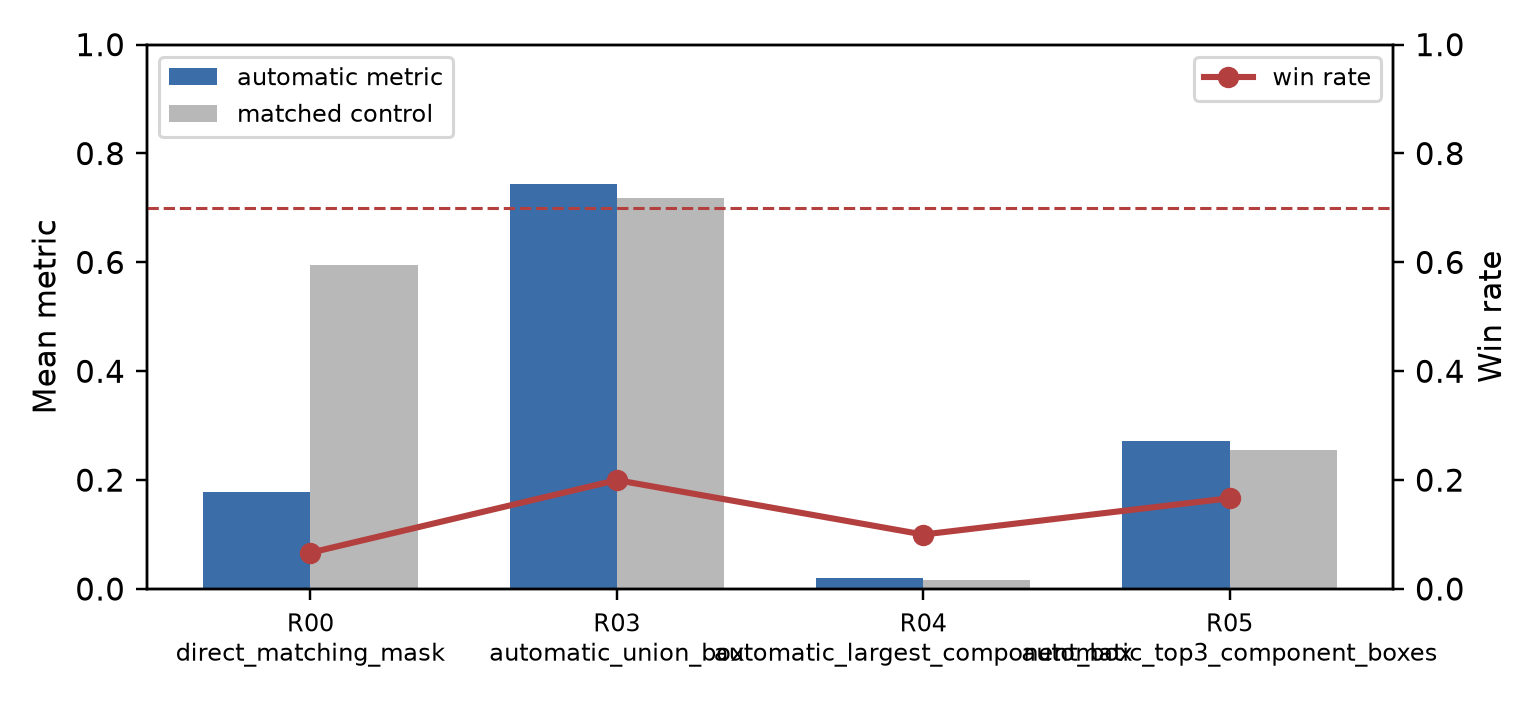
\includegraphics[width=.48\textwidth]{figures/r1_family_metrics.png}
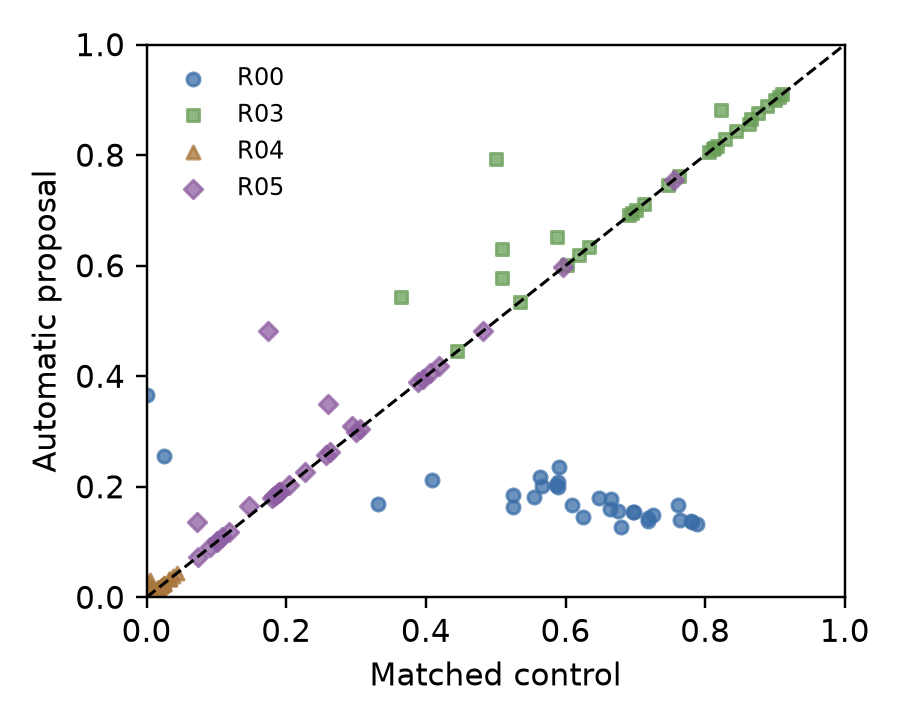
\includegraphics[width=.48\textwidth]{figures/r1_automatic_vs_control_scatter.png}
\caption{Gate R1 diagnostics. Left: automatic proposal metrics and matched controls by family, with the 0.70 win-rate threshold shown. Right: query-level automatic-versus-control scatter; most points do not clear the diagonal by a meaningful margin.}
\label{fig:r1_diagnostics}
\end{figure*}

\begin{figure}[t]
\centering
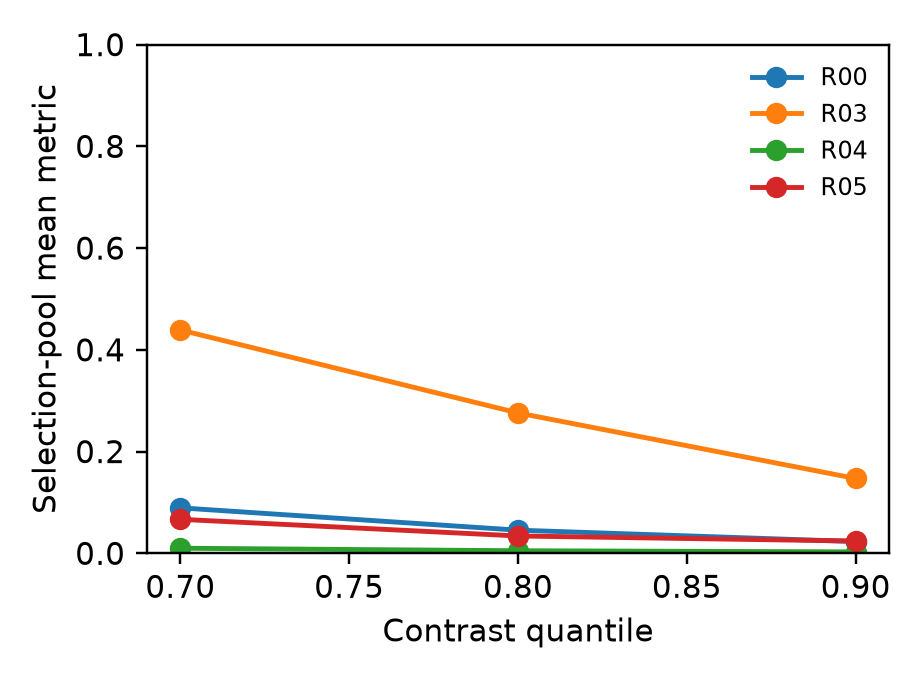
\includegraphics[width=\columnwidth]{figures/r1_parameter_grid_curves.png}
\caption{Internal selection-pool parameter grid summary. The selected configurations use the fixed pre-registered grid; strict validation is not used to choose parameters.}
\label{fig:r1_grid}
\end{figure}

\subsection{Blocked Downstream Quantities}

Because R1 fails before new SAM region inference, SAM-refined Dice, SAM gain, upper-bound recovery, R3 oracle gap, router comparison, and formal test results are not measured. Table~\ref{tab:downstream_status} records these as blocked quantities, not missing favorable results.

\begin{table*}[t]
\centering
\small
\caption{Downstream Phase 3 quantities are explicitly blocked by R1 failure rather than silently omitted.}
\label{tab:downstream_status}
\begin{tabular}{lll}
\hline
Stage & State & Reported value \\
\hline
R2 SAM region viability & BLOCKED\_BY\_R1\_FAILURE & not run \\
SAM gain & BLOCKED\_BY\_R1\_FAILURE & N/A \\
Region recovery & BLOCKED\_BY\_R1\_FAILURE & N/A \\
R3 oracle gap & BLOCKED\_BY\_R1\_FAILURE & N/A \\
Router & PROHIBITED\_BY\_R1\_FAILURE & not trained \\
Formal test & PROHIBITED\_BY\_R1\_FAILURE & testA/testB locked \\
\hline
\end{tabular}
\end{table*}

\begin{table*}[t]
\centering
\small
\caption{Compute, access, and final-state ledger for Phase 3.}
\label{tab:compute_access}
\begin{tabular}{ll}
\hline
Item & Value \\
\hline
Phase 3 GPU hours & 0.029398 \\
Budget & 40 \\
testA & LOCKED\_UNUSED \\
testB & LOCKED\_UNUSED \\
Preregistration commit & 471f529 \\
Final state & STOP\_GLAS\_REGION\_PROPOSAL\_FAILURE \\
\hline
\end{tabular}
\end{table*}

